\section{The Limit}\label{sec:LimitsWorkingDefn}
The value a function $f$ approaches as its input $x$ approaches some value is said to be the limit of $f$. Limits are essential to the study of calculus and, as we will see, are used in defining continuity, derivatives, and integrals.

Consider the function
$$f(x)=\frac{x^2-1}{x-1}.$$

Notice that $x=1$ does not belong to the domain of $f(x)$.
Regardless, we would like to know how $f(x)$ behaves close to the point $x=1$.
We start with a table of values:
$$\begin{array}{ccc}
\underline{x}&\qquad&\underline{f(x)}\\
0.5&\qquad&1.5\\
0.9&\qquad&1.9\\
0.99&\qquad&1.99\\
1.01&\qquad&2.01\\
1.1&\qquad&2.1\\
1.5&\qquad&2.5\\
\end{array}$$

It appears that for values of $x$ close to $1$ we have that $f(x)$ is close to $2$.
In fact, we can make the values of $f(x)$ as close to $2$ as we like by taking $x$ sufficiently close to $1$.
We express this by saying \ifont{the limit of the function $f(x)$ as $x$ approaches $1$ is equal to $2$} and use the notation:
$$\lim_{x\to 1}f(x)=2.$$
\begin{definition}{Limit (Useable Definition)}{Limit}
In general, we will write
$$\lim_{x\to a}f(x)=L,$$
if we can make the values of $f(x)$ arbitrarily close to $L$ by taking $x$ to be sufficiently close to $a$ (on either side of $a$) but not equal to $a$.
\end{definition}

We read the expression $\lim_{x\to a}f(x)=L$ as ``\ifont{the limit of $f(x)$ as $x$ approaches $a$ is equal to $L$}".
When evaluating a limit, you are essentially answering the following question: 
What number does the function \ifont{approach} while $x$ gets closer and closer to $a$ (but \ifont{not equal} to $a$)?
The phrase \ifont{but not equal to $a$} in the definition of a limit means 
that when finding the limit of $f(x)$ as $x$ approaches $a$ we never actually consider $x=a$.
In fact, as we just saw in the example above, $a$ may not even belong to the domain of $f$.
All that matters for limits is what happens to $f$ close to $a$, not necessarily what happens to $f$ at $a$.

\subsection*{One-sided limits}
Consider the following piecewise defined function:
%$$f(x)=
%\left\{\begin{array}{ccc}
%x,&\quad&\mbox{if $x\leq 1$,}\\
%x+1,&\quad&\mbox{if $x>1$,}\\
%\end{array}\right.$$
%which has the following visual representation:
$$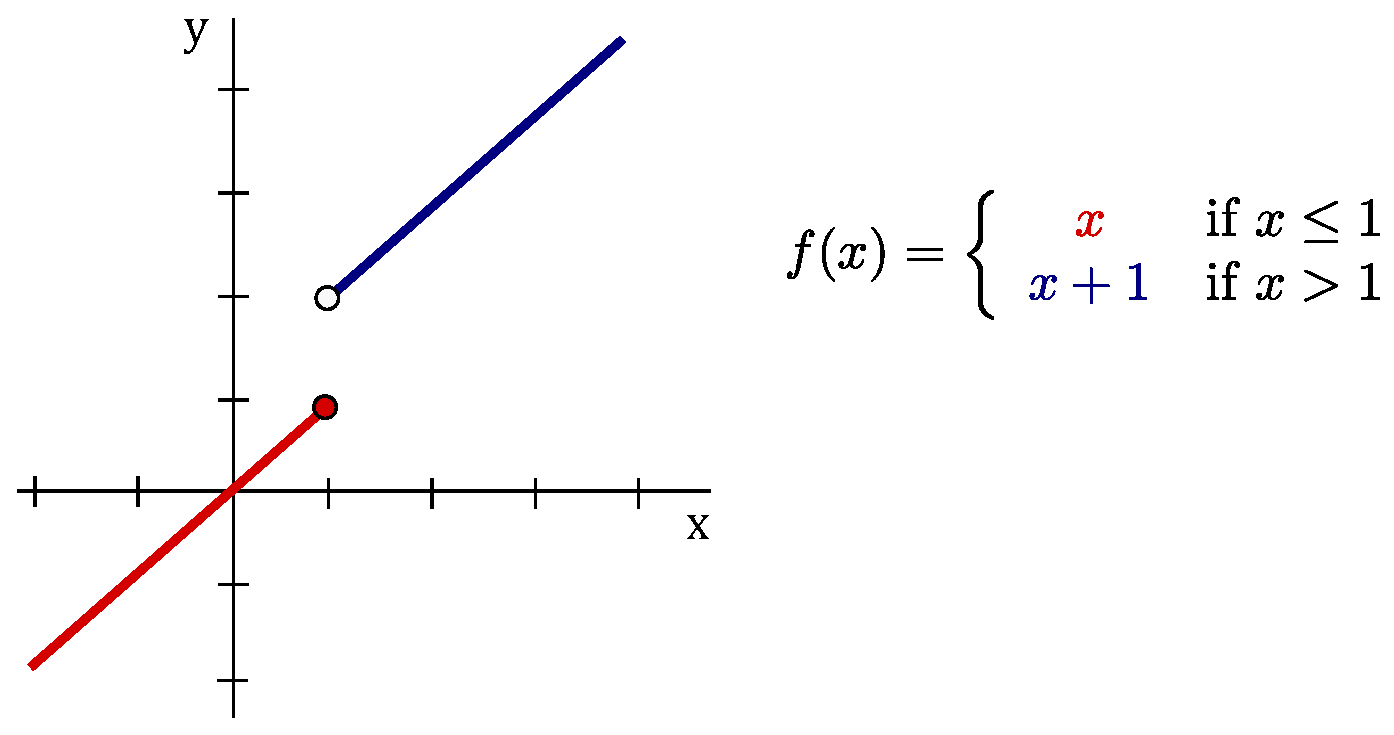
\includegraphics[width=4.0in]{images/limits-1}$$ Observe from the
graph that as $x$ gets closer and closer to $1$ from the \ifont{left},
then $f(x)$ approaches $+1$.  Similarly, as $x$ gets closer and closer
$1$ from the \ifont{right}, then $f(x)$ approaches $+2$.  We use the
following notation to indicate this: $$\lim_{x\to
1^-}f(x)=1\qquad\mbox{and}\qquad\lim_{x\to 1^+}f(x)=2.$$ The symbol
$x\to 1^-$ means that we only consider values of $x$ sufficiently
close to $1$ which are less than $1$.  Similarly, the symbol $x\to
1^+$ means that we only consider values of $x$ sufficiently close to
$1$ which are greater than $1$.

\begin{definition}{Left and Right-Hand Limit (Useable Definition)}{LeftRightHandLimit}
In general, we will write
$$\lim_{x\to a^-}f(x)=L,$$
if we can make the values of $f(x)$ arbitrarily close to $L$ by taking $x$ to be sufficiently close to $a$ and $x$ less than $a$.
This is called the \dfont{left-hand limit} of $f(x)$ as $x$ approaches $a$.
Similarly, we write
$$\lim_{x\to a^+}f(x)=L,$$
if we can make the values of $f(x)$ arbitrarily close to $L$ by taking $x$ to be sufficiently close to $a$ and $x$ greater than $a$.
This is called the \dfont{right-hand limit} of $f(x)$ as $x$ approaches $a$.
\end{definition}

We note the following fact:
\begin{center}
$\ds{\lim_{x\to a}f(x)=L\qquad\mbox{if and only if}\qquad\lim_{x\to a^-}f(x)=L\qquad\mbox{and}\qquad\lim_{x\to a^+}f(x)=L}.$
\end{center}
Or more concisely:
\[\lim_{x\to a^-}f(x)=\lim_{x\to a^+}f(x)=L\].
A consequence of this fact is that if the one-sided limits are \ifont{different}, then the two-sided limit $\ds{\lim_{x\to a}f(x)}$ does not exist, often denoted as: (DNE).

%%%%%%%%%%%%%%%%%%%%%%%%%%%%%%%%%%%%%%%%%%%%
\Opensolutionfile{solutions}[ex]
\section*{Exercises for Section \ref{sec:LimitsWorkingDefn}}

\begin{enumialphparenastyle}

%%%%%%%%%%
\begin{ex}
Use a calculator to estimate $\ds\lim_{x\to 0}
\frac{\sin x}{x}$, where $x$ is in radians.
\end{ex}

%%%%%%%%%%
\begin{ex}
Use a calculator to estimate $\ds\lim_{x\to 0}
\frac{\tan(3x)}{\tan(5x)}$, where $x$ is in radians.
\end{ex}

%%%%%%%%%%
\begin{ex}
Use a calculator to estimate $\ds\lim_{x\to 1^{+}}\frac{|x-1|}{1-x^2}$ and $\ds\lim_{x\to 1^{-}}\frac{|x-1|}{1-x^2}$.
\end{ex}

\end{enumialphparenastyle}